\subsection{Far field}
\begin{frame}{Far field}
    \begin{columns}
        \column{0.5\textwidth}
        Condition: \( r > L^2/2\lambda \) and \( r > 5 \lambda \)
        
        \begin{itemize}
            \item Electromagnetic fields:
        \end{itemize}
        \vspace{-2mm}
        \begin{align*}
            \mathbf{E} &= \dfrac{IL}{4 \pi} j \omega \mu \dfrac{ \exp ( - j \beta r) }{r} \sin \theta \mathbf{ \hat{\theta} }, \\
            \mathbf{H} &= \dfrac{IL}{4 \pi} j \beta \dfrac{ \exp ( - j \beta r) }{r} \sin \theta \mathbf{ \hat{\phi} }.
        \end{align*}

        \begin{itemize}
            \item Poynting vector:
        \end{itemize}
        \begin{equation*}
            \mathbf{S} = \dfrac{1}{2} \left( \dfrac{IL}{4 \pi} \right)^2 \omega \mu \beta \dfrac{\sin^2 \theta}{r^2} \mathbf{\hat{r}}.
        \end{equation*}
        
        \vspace{3mm}
        % In the far field, electromagnetic wave is the Spherical wave.
        \column{0.5\textwidth}
        \vspace{-6mm}
        \begin{itemize}
            \item Radiation loss power:
        \end{itemize}
        \begin{equation*}
            P_f = \iint \mathbf{S} \cdot \mathrm{d} \mathbf{s} = \dfrac{\omega \mu \beta}{12\pi} (I L)^2.
        \end{equation*}
        \vspace{-3mm}
        \begin{figure}
            \centering
            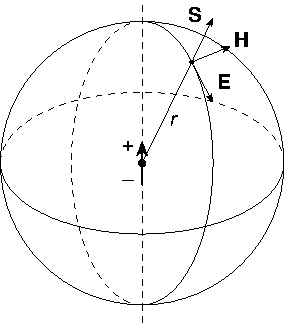
\includegraphics[width=0.75\textwidth]{Figures/Spherical_wave.pdf}
            \caption{Radiation in far fields.}
            \label{fig:Spherical_wave}
        \end{figure}
    \end{columns}
\end{frame}